\documentclass[conference]{IEEEtran}
\IEEEoverridecommandlockouts
\usepackage[T1]{fontenc}
\usepackage{cite}
\usepackage{amsmath,amssymb,amsfonts}
\usepackage{algorithmic}
\usepackage{graphicx}
\usepackage{textcomp}
\usepackage{xcolor}
\usepackage{bbm}
\usepackage{balance}
\usepackage{url}
\usepackage{amsmath}
\def\BibTeX{{\rm B\kern-.05em{\sc i\kern-.025em b}\kern-.08em T\kern-.1667em\lower.7ex\hbox{E}\kern-.125emX}}
\begin{document}

\title{Cost-Efficient Adaptive Routing for Human-in-the-Loop Email Assistants}

\author{\IEEEauthorblockN{<<Full Name>>}
\IEEEauthorblockA{<<Affiliation, City, Country>>\\
<<email>>}
}

\maketitle

\begin{abstract}
Invoking a large language model for every incoming email is expensive: a one-word acknowledgment costs as much to process as a nuanced complaint. We present an adaptive routing system that classifies email into seven categories and dispatches each message to the least expensive capable handler --- a template, an exact-match cache, FAQ retrieval, a calendar integration, a large LLM, or a spam handler --- with every side effect staged for human approval. On a 363-email synthetic corpus under stratified five-fold cross-validation, a fine-tuned DistilBERT classifier attains 92.29\% accuracy and 0.921 macro-F1, against 84.57\% for a TF-IDF linear SVM and 39.67\% for a frozen rule set, and cuts LLM cost 38.53\%. Measured cost reduction overstates what correct routing achieves: only 13.57 of the rule set's 28.98 points are attributable to correctly routed email, and the SVM's larger measured saving reverses once misroutes are excluded. On a held-out corpus of 105 emails generated by a different model and double-annotated (Cohen's $\kappa=0.900$), DistilBERT reaches 84.76\% and the SVM 85.71\%, statistically indistinguishable (exact McNemar $p=1.00$). Both corpora are synthetic; generalisation to human-written email remains untested.
\end{abstract}

\begin{IEEEkeywords}
adaptive routing, email classification, LLM cost reduction, DistilBERT, human-in-the-loop, retrieval-augmented generation
\end{IEEEkeywords}

\section{Introduction}
Email remains a primary channel for professional communication, and estimates put worldwide daily volume above 300 billion messages \cite{b1}. Assistants that read, classify and draft replies to that traffic are an active area of system design, though recent work finds that general-purpose LLM interfaces often miss the tone and interpersonal context an effective reply requires, and proposes explicit scaffolding to supply it \cite{b2}. Deploying one uniformly, however, is costly. Frontier models are priced per token, so a system that sends every message to a large LLM pays the same reasoning cost for a two-word acknowledgment as for a distressed complaint. At the scale of a professional inbox this compounds quickly.

Adaptive routing inserts a classification layer ahead of the handler layer: acknowledgments from a fixed set of prefabricated replies \cite{b3}, FAQ-style questions from a curated retrieval store, in the spirit of work answering customer-service questions from structured records of past issues \cite{b4}, repetitive support queries from cache \cite{b5}, and only messages requiring genuine generation reach the LLM \cite{b6}\cite{b7}. The saving depends on what fraction of traffic the inexpensive handlers absorb, and therefore on classification accuracy.

This paper makes three contributions: (1) a working adaptive routing pipeline for email, implemented with LangGraph \cite{b8} and connected to a live Gmail inbox, that classifies messages into seven categories and dispatches each to one of six handlers under human-approval constraints; (2) an out-of-fold evaluation supplemented by a separately generated, double-annotated ($\kappa = 0.900$) held-out corpus, comparing a rule-based classifier and a TF-IDF linear-model baseline against a fine-tuned DistilBERT \cite{b9} classifier; and (3) attributable cost reduction, a metric separating savings produced by correct routing from savings produced by misrouting into handlers that consume no tokens, together with evidence that the two differ substantially.

Our research questions are: (RQ1) How much can adaptive routing reduce LLM token usage, monetary cost and response latency relative to a baseline that always invokes a single large LLM? (RQ2) How much of a routed system's measured cost reduction is attributable to correct routing, rather than to misrouting into inexpensive handlers?

\section{Related Work}

\subsection{Prior Work}
Early email classifiers induced keyword-spotting rules over message text\cite{b10}: interpretable and fast, but brittle to phrasing variation --- a limitation we observe in our own rule-based baseline. \cite{b11} show DistilBERT embeddings with neural classifiers perform strongly on email spam detection, and fine-tuned BERT-family models are now standard for short-text classification \cite{b12}\cite{b13}.

Routing queries to the most cost-effective model has attracted significant recent attention. FrugalGPT \cite{b6} proposes a cascade in which cheaper models are tried first and queries escalate only when confidence is low. Hybrid LLM \cite{b7} trains a binary router on predicted difficulty. RouteLLM \cite{b14} learns routing policies from human preference data, BEST-Route \cite{b15} extends this with test-time optimal compute allocation, and Route to Reason \cite{b16} routes between inference and explicit reasoning strategies. Concurrent work on cascaded, clustering-based serving \cite{b17} explores similar cost-aware policies at larger scale. We extend these principles to the email domain and beyond LLM-to-LLM selection, to non-LLM handlers --- templates, caches, retrieval and calendar APIs --- that eliminate model invocation entirely for well-defined message types.

Lewis et al. \cite{b18} introduced RAG for grounding model outputs in external knowledge. We apply retrieval as a cost-reduction rather than quality-enhancement mechanism: where a curated answer exists, similarity search returns it verbatim, avoiding model invocation.

\section{System Design}

\subsection{Pipeline}
The pipeline has three sequential layers, shown in Fig.~\ref{fig1}: a Gmail poller that fetches unread messages at a configurable interval; a classifier that assigns each message to one of seven categories; and a handler layer that produces a response using the method appropriate to that category.\footnote{Code and data: \url{https://github.com/assem449/agentic-email-system}} Spam is a routing destination rather than a pre-pipeline filter --- messages the classifier labels spam terminate at a handler that blocks them and generates no reply --- so the spam figures reported in Section V measure classifier accuracy on that category and not the accuracy of an independent filter. Every routing decision, handler invocation, token count and latency is logged.

\begin{figure}[htbp]
\centerline{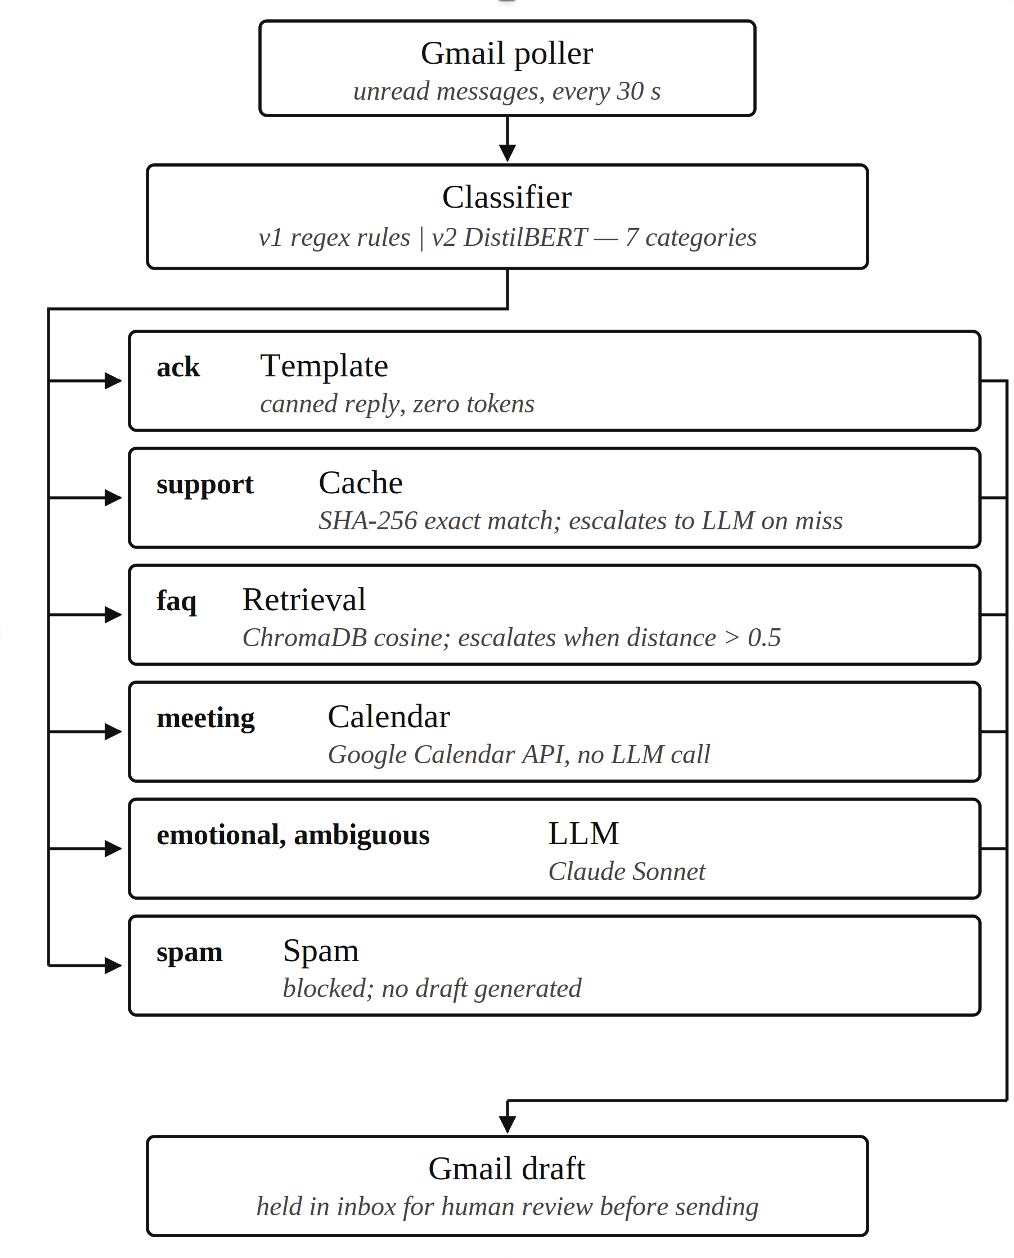
\includegraphics[width=0.85\linewidth]{fig1.png}}
\caption{Pipeline architecture. Each handler is listed with the category that routes to it. The cache escalates to the LLM on a miss, and retrieval escalates when the cosine distance to the nearest stored question exceeds the 0.5 threshold.}
\label{fig1}
\end{figure}

\subsection{Handlers}
\begin{itemize}
\setlength\itemsep{2pt}
\item \textbf{Template.} Acknowledgments are answered from a small lookup table keyed on the detected phrase. No model is invoked; latency is sub-millisecond and token cost is zero.
\item \textbf{Cache.} Support emails are normalised and hashed with SHA-256. A matching hash returns the stored response at $O(1)$ cost; a miss escalates to the LLM and the reply is stored. Matching is exact rather than semantic: paraphrases hash differently and count as misses.
\item \textbf{Retrieval.} FAQ-style emails are matched against a ChromaDB store of curated question-answer pairs, configured for cosine distance rather than the default squared L2; for unit-normalised embeddings the two are related by \eqref{eq1}, so a squared-L2 threshold of 1.0 and a cosine threshold of 0.5 select identical neighbours. Within the threshold the stored answer is returned verbatim; queries exceeding it fall back to the LLM. The threshold was fixed a priori rather than tuned.
\item \textbf{Calendar.} Scheduling requests are parsed for a proposed time using the \texttt{dateutil} library. The handler performs no write: it stages a pending record and returns a draft stating the extracted time for confirmation.
\item \textbf{LLM.} Emotional, nuanced and ambiguous messages reach Claude Sonnet 4.6 under a fixed system prompt instructing concise, empathetic replies without unverifiable commitments. Input and output token counts are recorded separately from the API response.
\item \textbf{Spam.} Blocked; no draft, no model call.
\end{itemize}

\begin{equation}
d_{l2}^{2}(q,v) = \lVert q - v \rVert_2^2 = 2\bigl(1-\cos(q,v)\bigr) = 2\,d_{\cos}(q,v)
\label{eq1}
\end{equation}

\subsection{Human Oversight and Threat Model}
A handler's output is staged rather than committed: replies are written as Gmail drafts and proposed meetings as pending records keyed by a confirmation token, so committing either requires an explicit user action, and the confirmation endpoint is idempotent, so a repeated confirmation cannot double-book. We assume an adversary who can send arbitrary email to the inbox but has no access to system internals. Because side-effecting handlers stage rather than commit, a misroute produces a discardable proposal, not a sent message or booked appointment. Prompt injection is not mitigated, though no handler exposes tool use, so an injected instruction cannot reach the mailbox directly. The largest unmitigated risk is adversarial cost inflation --- messages phrased to force LLM escalation --- which rate limiting or a budget ceiling would address; neither is implemented.

\section{Method}

\subsection{Implementation}
The system is implemented in Python 3.9. LangGraph \cite{b8} orchestrates the pipeline as a typed state graph in which classification, handler dispatch and logging are nodes, and conditional edges route state to the matching handler. The compiled graph is exposed through FastAPI. The Gmail poller fetches unread messages every 30 seconds and creates drafts through the Gmail Drafts API; the Calendar API is called only from the confirmation endpoint. ChromaDB runs locally in-memory for retrieval, and the cache is an in-memory dictionary with Redis as the intended production backend.

\subsection{Classifier Evaluation}
The v1 classifier applies a prioritised list of regular expressions to the lowercased concatenation of subject and body, in a deliberate evaluation order that checks acknowledgment patterns before meeting keywords. The v2 classifier fine-tunes \texttt{distilbert-base-uncased} \cite{b9} on the same concatenation, tokenized to a maximum length of 128. As an intermediate baseline we train two linear classifiers on TF-IDF
features (word unigrams and bigrams, sublinear term frequency) of the same
concatenation: multinomial logistic regression and a linear SVM, both with
$C{=}1$ and no tuning. The vocabulary is fitted within each training fold,
and both use the same five folds as DistilBERT, so all three trained
classifiers are compared on identical out-of-fold predictions.

Because the classifier is trained and evaluated on the same corpus, we use stratified $K$-fold cross-validation with out-of-fold prediction (an earlier version of this work scored an 80/20-split model over the full corpus, so 80\% of its reported accuracy had been seen in training): the corpus is partitioned into $K=5$ label-stratified folds, and for each fold $k$ a model trained on the other $K-1$ folds predicts only the emails in fold $k$, giving one out-of-sample prediction per email. Writing $N$ for the corpus size, $\kappa(i)$ for the fold containing email $i$ and $\mathbbm{1}[\cdot]$ for the indicator function, pooled out-of-fold accuracy is \eqref{eq2}. Each fold trains for 10 epochs at batch size 8, roughly 64 seconds on a laptop CPU.

\begin{equation}
\mathrm{Acc}_{\mathrm{OOF}}
=
\frac{1}{N}
\sum_{i=1}^{N}
\mathbbm{1}\bigl[f_{\kappa(i)}(x_i)=y_i\bigr]
\label{eq2}
\end{equation}

The rule set is not trained, but its expressions were revised across several cycles while inspecting evaluation results on an earlier version of this corpus, so it was effectively fitted by hand. It is frozen for all results below: fixed before the expanded corpus was generated and unmodified afterwards.

\subsection{Metrics}
We report routing accuracy, macro-F1 with per-category precision and recall, token reduction, cost reduction and latency reduction against an always-LLM baseline that routes every message directly to the LLM. Token and cost reduction are reported separately because they are not the same quantity: output tokens are billed at five times the input rate for the model used here (\$3.00 and \$15.00 per million input and output tokens respectively, at the rates in effect during evaluation \cite{b19}), so writing T and p for token totals and prices per million tokens, cost follows \eqref{eq3} and coincides with token reduction only when routing removes both directions in the same proportion, which it does not.

\begin{equation}
C =
\frac{T_{\mathrm{in}}p_{\mathrm{in}} +
T_{\mathrm{out}}p_{\mathrm{out}}}{10^6}
\label{eq3}
\end{equation}

Measured cost reduction counts every token the routed system avoided spending, whether or not the handler that avoided them was the one designated by the ground-truth routing policy for that message. To separate these we define attributable cost reduction: for each email $i$ the saving is the difference between what the baseline paid and what the routed system paid, and \eqref{eq4} sums those savings over correctly routed emails only, normalised by total baseline cost. The difference between the measured and attributable figures is the portion of a system's apparent savings produced by sending mail to handlers that consume no tokens because they were not the handlers designated by the ground-truth routing policy.

\begin{equation}
R_{\mathrm{attr}}
=
\frac{
\sum_{i \in \mathcal{C}}
\left(C_{\mathrm{base},i} - C_{\mathrm{route},i}\right)
}{
\sum_{i=1}^{N} C_{\mathrm{base},i}
}
\label{eq4}
\end{equation}

\section{Results}

\subsection{Dataset}
The evaluation corpus consists of 363 labelled emails: support (67), acknowledgment (52), ambiguous (52), FAQ (50), emotional (50), meeting request (47) and spam (45). It is synthetic, generated under seven category-specific prompts requesting canonical phrasings, natural paraphrases and trap cases that probe known failure modes --- an acknowledgment containing the word ``meeting'', a support request phrased as a question --- extending to in-scope messages the motivation Larson et al.~\cite{b20} give for evaluating beyond examples that sit comfortably inside a label. Every figure below is a result on synthetic correspondence.

\paragraph{Generation details.} The primary corpus was generated with Claude Sonnet~5 (Anthropic) and the held-out corpus with GPT-4o (OpenAI), both in August 2026 through the vendors' chat interfaces at default settings, so the corpora differ in model and vendor as well as in prompts. Each came from seven category-specific role-play prompts (``Imagine you are\ldots'') specifying the category and a sender persona and requesting canonical phrasings, natural paraphrases and a minority of trap cases. The verbatim prompts were not retained; approximate reconstructions, written after the fact and not the original text, are released with the corpora, labels and adjudication record. Replies on the LLM path come from Claude Sonnet~4.6, which generated neither corpus.

\subsection{Label Provenance and Validation}
Ground-truth labels are not the generator's: the category a prompt requested was treated as a proposal only. Emails were deduplicated and every email in both corpora was labelled by hand by one author; trap cases carry the label of their intent, not of the prompt that produced them. Messages genuinely undecidable between two functional categories were labelled ambiguous rather than discarded, which is part of why that category is both the largest source of classifier error and the hardest to define positively.

The 363 primary-corpus labels come from a single annotator, so its accuracies measure agreement with one reader's judgment; the ambiguous boundary in particular carries annotation uncertainty beyond the reported intervals, which capture sampling variation only. The held-out corpus, which carries the generalisation claim, was independently double-annotated by a second annotator blind to the original labels and prompts: raw agreement was 96/105 (91.4\%), Cohen's $\kappa = 0.900$. Of the 9 disagreements, 8 were trap cases; 6 were resolved in the second annotator's favour because their label matched the category the trap was built to disguise, and 3 by discussion. The adjudicated labels are the ground truth for every held-out figure.

\subsection{Routing Accuracy}
Table~\ref{tab1} compares DistilBERT against the always-LLM and random-routing baselines, the frozen rule set and the two TF-IDF classifiers. DistilBERT v2 attains 92.29\% pooled out-of-fold accuracy (335/363, 95\% CI 89.1--94.6); per-fold accuracies average 92.29\% with a standard deviation of 1.84\% (range 90.41--95.83\%), indicating the estimate is not an artifact of a favourable partition. Accuracy intervals throughout are Wilson score intervals at 95\%; macro-F1 intervals are bootstrap percentile intervals over 10,000 resamples. On the primary corpus DistilBERT v2 attains macro-F1 0.921 (95\% CI 0.891--0.947) against 0.386 (0.333--0.435) for the frozen rule set. This is well below the 98.45\% reported when the same model was scored on data it had trained on (Section IV-B). Random routing scores 11.85\%, close to the 14.3\% expected by chance.

\begin{table}[htbp]
\caption{Routing Systems on the 363-Email, Seven-Category Corpus}
\begin{center}
\setlength{\tabcolsep}{1.8pt}
\renewcommand{\arraystretch}{0.75}
\begin{tabular}{|l|c|c|c|c|c|}
\hline
\textbf{System} & \textbf{Acc.} & \textbf{Macro-F1} & \textbf{Tok. red.} & \textbf{Cost red.} & \textbf{Lat. red.} \\
\hline
Always-LLM (baseline) & --- & --- & 0\% & 0\% & 0\% \\
\hline
Random routing & 11.85\% & 0.116 & --- & --- & --- \\
\hline
Rules v1 (frozen) & 39.67\% & 0.386 & 29.28\% & 28.98\% & 29.23\% \\
\hline
TF-IDF + LR (OOF) & 79.06\% & 0.792 & 34.17\% & 33.57\% & 33.28\% \\
\hline
TF-IDF + SVM (OOF) & 84.57\% & 0.842 & 41.49\% & 40.71\% & 41.08\% \\
\hline
DistilBERT v2 (OOF) & 92.29\% & 0.921 & 39.47\% & 38.53\% & 36.72\% \\
\hline
\noalign{\vskip 3pt}
\multicolumn{6}{l}{\footnotesize Trained classifiers are scored out-of-fold per \eqref{eq2}; rules v1 is evaluated} \\
\multicolumn{6}{l}{\footnotesize frozen. Cost is computed per \eqref{eq3}. Latency is end-to-end (classifier} \\
\multicolumn{6}{l}{\footnotesize inference plus handler), including calendar-routed emails, whose handler} \\
\multicolumn{6}{l}{\footnotesize is stubbed during evaluation.}
\end{tabular}
\label{tab1}
\end{center}
\end{table}

The linear baselines close most of the gap: TF-IDF with a linear SVM attains 84.57\% (95\% CI 80.5--87.9) and macro-F1 0.842 (0.802--0.878), logistic regression 79.06\% and 0.792. DistilBERT's 7.72-point lead over the SVM lies outside both intervals, but 44.90 of the 52.62 points separating DistilBERT from the rules are recovered by a bag-of-words model that classifies an email in about 0.3~ms on CPU.

The rule-based classifier had previously reached 94.57\% on the corpus against which it was iteratively patched. Evaluated frozen on the expanded corpus it reaches 39.67\%. Nothing about the rule set changed between those measurements; only the corpus did. The 54.90-point collapse measures how much of a hand-tuned classifier's apparent accuracy can consist of fitting to the specific phrasings it was shown during development. This is training-set leakage arriving through manual engineering rather than gradient descent, and easy to miss: no training run occurs, so there is no obvious point at which to ask whether the evaluation is held out.

Table~\ref{tab2} gives per-category precision, recall and F1. Macro-F1 separates the classifiers more sharply than accuracy, because accuracy can be carried by larger categories while a smaller one is effectively abandoned. Rules v1 reaches 0.386: on spam it attains precision 0.667 against recall 0.089, correctly blocking 4 of 45 spam emails, and on emotional precision 0.917 against recall 0.220. In both the rules fire rarely and are reliable when they do, which accuracy conceals. DistilBERT v2 shows the opposite profile: 0.921 macro-F1 with no category below 0.845. Its errors concentrate in the ambiguous category, which accounts for 11 of 28 errors; that label is defined negatively, as the residual for messages not clearly belonging to a functional category, so it has no positive semantic signature to learn and its boundary with every other category is genuinely contested.

\begin{table}[htbp]
\caption{Per-Category Results on Both Corpora}
\begin{center}
\scriptsize
\setlength{\tabcolsep}{1.5pt}
\renewcommand{\arraystretch}{0.8}
\begin{tabular}{|l|cc|ccc|cc|ccc|}
\hline
& \multicolumn{5}{c|}{\textbf{Primary (363)}} & \multicolumn{5}{c|}{\textbf{Held-out (105)}} \\
\textbf{Category} & \textbf{n} & \textbf{Rules} & \multicolumn{3}{c|}{\textbf{DistilBERT}} & \textbf{n} & \textbf{Rules} & \multicolumn{3}{c|}{\textbf{DistilBERT}} \\
\cline{4-6} \cline{9-11}
& & \textbf{F1} & \textbf{P} & \textbf{R} & \textbf{F1} & & \textbf{F1} & \textbf{P} & \textbf{R} & \textbf{F1} \\
\hline
ack. & 52 & 0.627 & 0.943 & 0.962 & 0.952 & 13 & 0.703 & 0.812 & 1.000 & 0.897 \\
ambiguous & 52 & 0.305 & 0.911 & 0.788 & 0.845 & 18 & 0.436 & 0.737 & 0.778 & 0.757 \\
emotional & 50 & 0.355 & 0.923 & 0.960 & 0.941 & 14 & 0.421 & 0.929 & 0.929 & 0.929 \\
FAQ & 50 & 0.351 & 0.939 & 0.920 & 0.929 & 14 & 0.222 & 0.812 & 0.929 & 0.867 \\
meeting & 47 & 0.444 & 0.882 & 0.957 & 0.918 & 14 & 0.467 & 0.824 & 1.000 & 0.903 \\
spam & 45 & 0.157 & 0.952 & 0.889 & 0.920 & 14 & 0.000 & 0.917 & 0.786 & 0.846 \\
support & 67 & 0.463 & 0.915 & 0.970 & 0.942 & 18 & 0.703 & 1.000 & 0.611 & 0.759 \\
\hline
\textbf{macro} & 363 & 0.386 & 0.924 & 0.921 & 0.921 & 105 & 0.422 & 0.862 & 0.862 & 0.851 \\
\hline
\noalign{\vskip 3pt}
\multicolumn{11}{l}{\scriptsize Rules F1 is the frozen rule set's F1; P/R/F1 are DistilBERT, out-of-fold on} \\
\multicolumn{11}{l}{\scriptsize the primary corpus and fine-tuned on all 363 primary emails for the held-out} \\
\multicolumn{11}{l}{\scriptsize corpus (n = 105, generated by a different model, GPT-4o). Rule-set precision} \\
\multicolumn{11}{l}{\scriptsize and recall are given in prose. Held-out category counts are non-uniform} \\
\multicolumn{11}{l}{\scriptsize because trap cases carry labels differing from the prompt that generated them.}
\end{tabular}
\label{tab2}
\end{center}
\end{table}

\subsection{Cost and Latency}
Against an always-LLM baseline of 81,769 tokens (44,489 input, 37,280 output) costing \$0.6927, the routed pipeline under DistilBERT v2 consumes 49,492 tokens at \$0.4257: a 39.47\% reduction in tokens, 38.53\% in cost and 36.72\% in end-to-end latency --- at the observed rates, \$1,910 per million emails reduced to \$1,170. Cost reduction falls below token reduction because the routed output share rises from 45.6\% to 46.7\%. Latency in Table~I is end-to-end: classifier inference plus handler time, excluding Gmail I/O. DistilBERT inference takes a median 14.1~ms per email benchmarked on a laptop CPU (2.0~s one-off model load) and averages 40.8~ms inside the pipeline, where it runs on a CPU idled by multi-second API waits; the TF-IDF and rule classifiers take under 3~ms. Under the in-pipeline figures used in Table~I, inference lowers DistilBERT's latency reduction from 38.00\% (handler only) to 36.72\%. Calendar latency is a lower bound: the handler is replaced by a fixed 0.1~ms stub during evaluation, and the live handler's date extraction is a naive fuzzy parse. Excluding the 51 calendar-routed emails, DistilBERT's end-to-end reduction is 27.49\% (SVM 32.00\%, rules 19.54\%).

\subsection{Held-Out Generalisation}
Out-of-fold prediction removes leakage between individual emails but not at the level of the generator: emails from one prompt are stylistic siblings, so a model could score well by recognising a prompt's output rather than learning the category, and cross-validation cannot tell the two apart. We therefore built a second corpus of 105 emails from reworded prompts with different senders, scenarios and registers, generated by a different model, 15 per prompt; after adjudication, true-category counts range from 13 (acknowledgment) to 18 (ambiguous and support) because trap cases carry labels differing from their prompt. The domain was held constant, so that any drop reflects the generator rather than domain shift, and the corpora share no text or identifiers. A single classifier was fine-tuned on all 363 primary emails, since a fold model would not represent the deployed system.

Accuracy is 84.76\% (89/105, 95\% CI 76.7--90.4) and macro-F1 0.851 (95\% CI 0.775--0.913), against 92.29\% and 0.921 (0.891--0.947) on the primary corpus, though the two are not directly comparable: the primary figure is out-of-fold across models each trained on roughly 80\% of the corpus, while the held-out figure comes from a single model trained on all 363. The accuracy intervals overlap only narrowly, 89.1--90.4, so the 7.53-point decline is a real signal, though its exact size should be read cautiously given that narrow overlap. The classifier comparison is unaffected: on the held-out corpus the rule set attains macro-F1 0.422 (0.331--0.500), an interval disjoint from DistilBERT's.

The linear baselines generalise differently. Refitted on all 363 primary emails, the SVM attains 85.71\% (90/105, 95\% CI 77.8--91.2) and macro-F1 0.860 (0.784--0.919) on the held-out corpus, and logistic regression 80.95\% and 0.814, neither declining from cross-validation. On the held-out corpus the SVM and DistilBERT are indistinguishable (exact McNemar test on paired predictions: 7 emails only DistilBERT gets right, 8 only the SVM; $p=1.00$), so DistilBERT's in-corpus lead does not survive a change of generator: part of what fine-tuning learned is the primary generator's style.

The right-hand half of Table~\ref{tab2} gives the per-category breakdown. The decline is concentrated in support, which falls from 0.942 to 0.759 F1, well beyond any other category; ambiguous, spam, FAQ and acknowledgment show a smaller decline of 0.055--0.088 F1, while meeting and emotional are essentially unchanged. Support recall falls to 0.611 against precision 1.000, so the classifier misses support emails rather than confusing them with a neighbouring category. The rule set moves the opposite way, rising to 48.57\% accuracy (51/105); a keyword matcher improving while a fine-tuned model declines points to more prototypical phrasing rather than uniformly greater difficulty, stronger evidence of robustness to generator variation than cross-validation alone provides, though not of generalisation to real inbox email.

\subsection{Handler Effectiveness}
Routing accuracy measures whether an email reaches the intended handler, not whether that handler was the one designated by the ground-truth routing policy, or how well it responded. The response cache achieved a hit rate of exactly zero (0/41 under rules v1, 0/71 under DistilBERT v2): a hit requires two emails to be character-identical after normalisation, and the corpus was deduplicated, so every support email escalated to the LLM. A non-zero rate would require repeated text, which deduplication removes by construction, or semantic matching, which this handler does not implement. The retrieval handler achieved 20.4\% under DistilBERT v2, answering 10 of the 49 emails routed to it and escalating 39 to the LLM; because the threshold was fixed a priori we cannot separate whether it is too strict or the store too small.

\section{Discussion}

\subsection{RQ1: Magnitude of the Reduction}
Adaptive routing reduces tokens by 39.47\%, cost by 38.53\% and latency by 36.72\% against always invoking the LLM. The saving originates in the template, calendar, spam and retrieval-hit paths, which consume no tokens, so its magnitude depends on what fraction of traffic those handlers absorb. Acknowledgments are the clearest case: 50 of the 52 are answered from a fixed template at zero token cost, and they are both frequent and trivially identifiable in real inboxes.

These are LLM-side savings only. Every draft is staged for human review, so an email's full cost also includes the time a person spends checking, correcting or discarding it, which we do not measure and which need not track token cost: a templated reply to a misrouted email is free to generate but may cost more to repair than an LLM draft. Cost figures also exclude the compute cost of running the classifier and retrieval embedding model locally. The planned user study (Section~VI-C) would supply the missing review-time term.

\subsection{RQ2: Attributable Cost Reduction}
Substantially less than the headline figures suggest. Applying \eqref{eq4}, only 13.57 of rules v1's 28.98 percentage points of measured cost reduction are attributable to correctly routed email: 53.2\% of its savings, \$0.1068 of \$0.2007, arise from emails it got wrong. DistilBERT v2 is far better behaved, with 35.78 of 38.53 points attributable and 7.2\% of savings from misroutes. Fig.~\ref{fig3} shows the contrast.

\begin{figure}[htbp]
\centerline{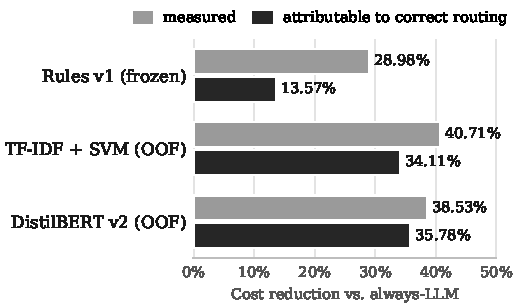
\includegraphics[width=\linewidth]{fig3.pdf}}
\caption{Measured cost reduction against the portion attributable to correctly routed email. More than half of the rule-based system's apparent savings come from misroutes; the TF-IDF SVM's measured lead over DistilBERT reverses once misroutes are excluded.}
\label{fig3}
\end{figure}

The mechanism is visible in the handler distribution. Rules v1 sends 119 emails to zero-token handlers, 55 of them misroutes, against 156 and 11 for DistilBERT v2. The concentration matters: 29 of the 55 land in the template handler and 23 in the calendar handler, precisely the paths where being wrong is most visible to a recipient. The cost metric records which handler ran, not whether that handler was the one the ground-truth policy designated, so tokens saved by a misroute count identically to those saved by a correct route.

Restricted to non-spam email the two classifiers are nearly indistinguishable on cost (29.15\% vs. 29.33\%) despite a 52.62-point accuracy gap; DistilBERT's full-corpus lead comes almost entirely from spam suppression (42 blocked vs. 6). Eq.~\eqref{eq4} credits a misroute with its full saving, slightly overstating the misrouted share, since a template reply to an ambiguous email is not necessarily a poor one.

The TF-IDF SVM makes the same point from the other direction. It shows the largest measured cost reduction of any system, 40.71\% against DistilBERT's 38.53\%, despite 7.72 points lower accuracy, because it sends more mail to zero-token handlers (163 against 156), 27 of them misrouted against 11. Only 34.11 of its points are attributable, below DistilBERT's 35.78: ranked by measured savings the SVM is the better router, ranked by attributable savings DistilBERT is. A cost comparison that does not separate the two can reward the less accurate router.

\subsection{Limitations and Future Work}
Both corpora are synthetic and 363 examples is small for fine-tuning. Three questions are left explicitly to future work. \emph{Response quality and review burden:} we measure whether an email reaches the intended handler, not whether its draft is acceptable; a planned user study will measure draft acceptance and editing effort per handler, supplying the human-review term missing from our cost accounting. \emph{Real email and annotation:} the held-out corpus (different model and vendor, reworded prompts, $\kappa = 0.900$) tests robustness to the generation process, not to real inbox traffic with its formatting noise and quoted threads; evaluation on consented real email, and double annotation of the single-annotated primary corpus, come next. \emph{Untuned components:} the retrieval threshold, cache design and rate limiting are fixed a priori or not yet implemented.

\section{Conclusion}
We presented an adaptive routing system for human-in-the-loop email assistance. Under five-fold cross-validation a fine-tuned DistilBERT classifier achieved 92.29\% routing accuracy and 0.921 macro-F1, against 39.67\% for a frozen rule set that had scored 94.57\% on the corpus it was tuned against, and reduced LLM cost 38.53\%. On a held-out corpus from a different model, double-annotated ($\kappa = 0.900$), it reached 84.76\%, statistically indistinguishable from a TF-IDF linear SVM, so routing accuracy on an unseen generator does not depend on a fine-tuned transformer. Our central methodological finding is that measured cost reduction overstates what correct routing achieves: only 13.57 of the rule set's 28.98 points are attributable to correctly routed email, against 35.78 of 38.53 for DistilBERT, and the SVM's larger measured saving reverses once misroutes are excluded. Cost savings alone are therefore not evidence that a router is working.

\section*{Acknowledgment}
All 363 primary and 105 held-out emails were generated by large language models (Section V-A); no real user correspondence was collected or analysed. Figures 1 and 2 were produced with the assistance of Claude (Anthropic); the authors specified their content, verified every technical detail against the implementation, and take full responsibility for their accuracy.

\balance
\begin{thebibliography}{00}
\footnotesize
\bibitem{b1} Radicati Group, ``Email Statistics Report, 2023-2027,'' The Radicati Group, Inc., Palo Alto, CA, USA, 2023.
\bibitem{b2} R. Yao et al., ``PersonaMail: Learning and Adapting Personal Communication Preferences for Context-Aware Email Writing,'' in Proc. 31st Int. Conf. Intelligent User Interfaces (IUI '26), Paphos, Cyprus, 2026, pp. 197-217.
\bibitem{b3} X. Zhu et al., ``Explicit and Implicit Semantic Ranking Framework,'' in Companion Proc. ACM Web Conf. 2023, Austin, TX, USA, 2023, pp. 326-330.
\bibitem{b4} Z. Xu et al., ``Retrieval-Augmented Generation with Knowledge Graphs for Customer Service Question Answering,'' in Proc. 47th Int. ACM SIGIR Conf. Research and Development in Information Retrieval, Washington, DC, USA, 2024, pp. 2905-2909.
\bibitem{b5} S. Regmi and C. P. Pun, ``GPT Semantic Cache: Reducing LLM Costs and Latency via Semantic Embedding Caching,'' arXiv:2411.05276, 2024.
\bibitem{b6} L. Chen, M. Zaharia, and J. Zou, ``FrugalGPT: How to Use Large Language Models While Reducing Cost and Improving Performance,'' arXiv:2305.05176, 2023.
\bibitem{b7} D. Ding et al., ``Hybrid LLM: Cost-Efficient and Quality-Aware Query Routing,'' in Proc. 12th Int. Conf. Learning Representations (ICLR), Vienna, Austria, 2024.
\bibitem{b8} LangChain Inc., ``LangGraph: Agent orchestration framework for LLMs,'' 2024. [Online]. Available: https://github.com/langchain-ai/langgraph. [Accessed: Aug. 26, 2026].
\bibitem{b9} V. Sanh, L. Debut, J. Chaumond, and T. Wolf, ``DistilBERT, a distilled version of BERT: smaller, faster, cheaper and lighter,'' arXiv:1910.01108, 2019.
\bibitem{b10} W. W. Cohen, ``Learning Rules that Classify E-Mail,'' in Papers from the AAAI Spring Symp. Machine Learning in Information Access, Tech. Rep. SS-96-05, Stanford, CA, USA, 1996, pp. 18-25.
\bibitem{b11} G. P. Reddy et al., ``An LLM driven framework for email spam detection using DistilBERT embeddings and neural classifiers,'' Discover Applied Sciences, vol. 8, no. 2, art. no. 146, 2026.
\bibitem{b12} J. Devlin, M.-W. Chang, K. Lee, and K. Toutanova, ``BERT: Pre-training of Deep Bidirectional Transformers for Language Understanding,'' in Proc. NAACL-HLT, Minneapolis, MN, USA, 2019, pp. 4171-4186.
\bibitem{b13} C. Sun, X. Qiu, Y. Xu, and X. Huang, ``How to Fine-Tune BERT for Text Classification?'' in Chinese Computational Linguistics: 18th China National Conf. (CCL 2019), Kunming, China, 2019, pp. 194-206.
\bibitem{b14} I. Ong et al., ``RouteLLM: Learning to Route LLMs from Preference Data,'' in Proc. 13th Int. Conf. Learning Representations (ICLR), Singapore, 2025.
\bibitem{b15} D. Ding et al., ``BEST-Route: Adaptive LLM Routing with Test-Time Optimal Compute,'' in Proc. 42nd Int. Conf. Machine Learning (ICML), Vancouver, Canada, 2025, vol. 267 of Proceedings of Machine Learning Research, pp. 13870-13884.
\bibitem{b16} Z. Pan, K. Zhang, Y. Zhao, and Y. Han, ``Route to Reason: Adaptive Routing for LLM and Reasoning Strategy Selection,'' arXiv:2505.19435, 2025.
\bibitem{b17} Y. Moslem et al., ``Cluster, Route, Escalate: Cascaded Framework for Cost-Aware LLM Serving,'' arXiv:2606.27457, 2026.
\bibitem{b18} P. Lewis et al., ``Retrieval-Augmented Generation for Knowledge-Intensive NLP Tasks,'' in Proc. NeurIPS, 2020.
\bibitem{b19} Anthropic, ``Pricing,'' Claude Platform Documentation. [Online]. Available: https://platform.claude.com/docs/en/about-claude/pricing. [Accessed: Aug. 28, 2026].
\bibitem{b20} S. Larson et al., ``An Evaluation Dataset for Intent Classification and Out-of-Scope Prediction,'' in Proc. EMNLP-IJCNLP, Hong Kong, China, 2019, pp. 1311-1316.
\end{thebibliography}

\end{document}
